\documentclass[a4paper, 13px]{article}
\usepackage{graphicx}
\usepackage[utf8]{inputenc}
\usepackage[T1]{fontenc}
\usepackage{geometry}
\usepackage{tcolorbox}
\usepackage{enumitem}
\usepackage{tocloft}
\usepackage{framed}


\geometry{a4paper, margin=2cm}

\begin{document}
\definecolor{myblue}{RGB}{0, 102, 204}
\newtcolorbox{mybox}{
    colframe=myblue,
    colback=white,
    arc=0pt,
    outer arc=0pt,
    boxrule=1pt,
    boxsep=0pt,
    left=10pt,
    right=10pt,
    top=10pt,
    bottom=10pt
}

\begin{center}
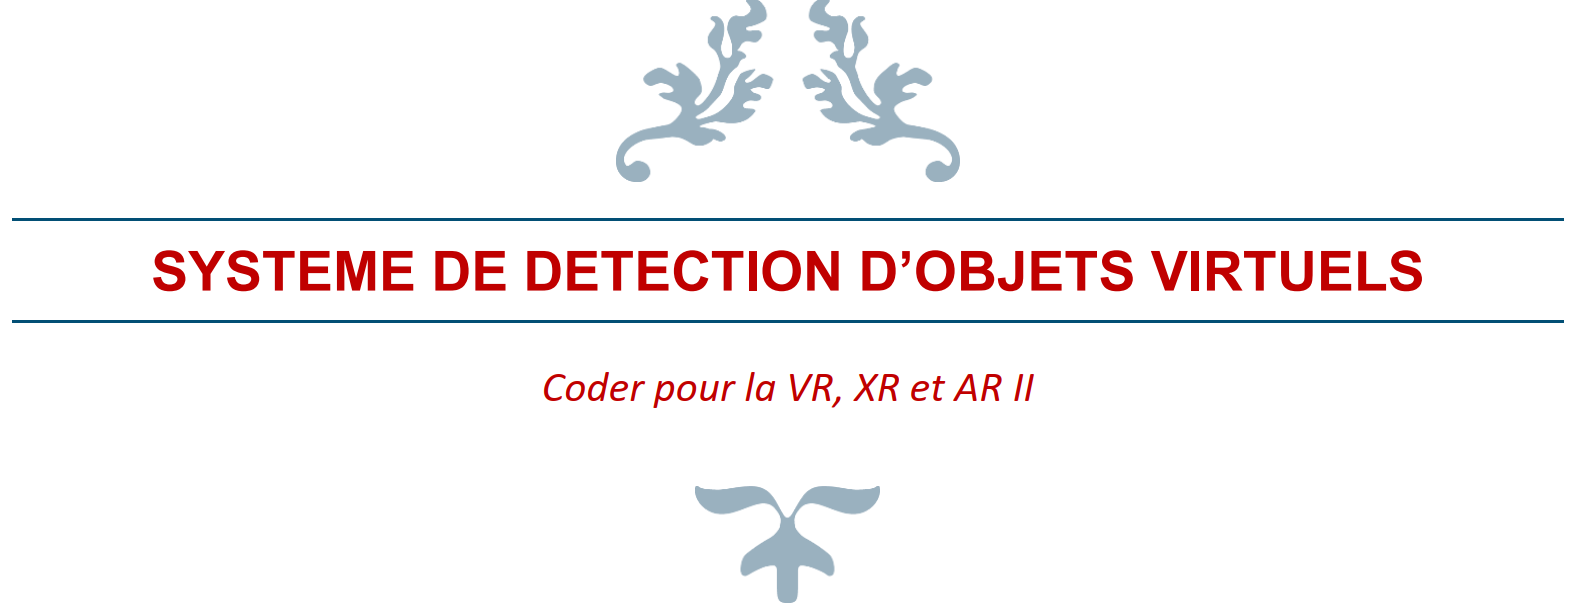
\includegraphics[scale=0.5]{im1.png}\\\




\large REALISE PAR\\
\begin{framed}
\large\bfseries{ ESSAM ETIENNE ERNEST 22P126}\\

{NGOA NTSAMA Yves Patrick Joel 22P129 }\\

{SIPA FRANCK 22P130}
\end{framed}
\end{center}



\newpage



\Large {\bfseries \underline{PLAN}}\\
\\
\begin{framed}
{\bfseries  INTRODUCTION}                                        \\
•	Contexte et objectifs du projet	                \\
•	Présentation de la technologie Yolo et de l'AR	\\
•	Importance de la détection d'objets virtuels	     \\
{\bfseries \MakeUppercase{I. Architecture du système  }}	                        \\
{\bfseries \MakeUppercase{II. Implémentation}}                                 \\
1-	Préparation de l'environnement de développement	\\
2-	Intégration de la caméra AR	                     \\
3-	Configuration du modèle Yolo	                     \\
•	Préparation des données :	                     \\
•	Architecture du modèle :	                         \\
•	Entraînement du modèle :	                         \\
4-	Intégration du système de détection dans Visual Studio Code	\\
{\bfseries \MakeUppercase{III. Résultats et évaluation}}	                         \\
a-	Métrique d’évaluation	                         \\
b-	Retour d'expérience des utilisateurs :	        \\
{\bfseries \MakeUppercase{ IV. Défis et limitations}}                          	\\
1.	Problèmes rencontrés lors du développement	    \\
2.	Limitations actuelles du système :	            \\
3.	Pistes d'amélioration future	                    \\
{\bfseries \MakeUppercase{Conclusion}}
\end{framed}



\newpage

{\bfseries  INTRODUCTION}\\

•	{\bfseries \underline{Contexte et objectifs du projet}}\\

La détection d'objets virtuels dans des environnements de réalité augmentée (AR) est de plus en plus importante pour de nombreuses applications, telles que le commerce en ligne, les jeux et la formation. Ce projet vise à développer un système de détection d'objets virtuels en temps réel, intégré à l'environnement de développement Visual Studio Code et utilisant l'algorithme de détection d'objets Yolo. L'objectif principal est de fournir aux développeurs une solution simple et efficace pour intégrer la détection d'objets virtuels dans leurs applications AR. Le système devra offrir des performances élevées en termes de précision et de rapidité de traitement, tout en étant facilement configurable et adaptable à divers scénarios d'utilisation. En exploitant les capacités de l'AR et de la détection d'objets avancée, ce projet cherche à repousser les limites actuelles de l'interaction entre les objets virtuels et le monde réel.\\

•	{\bfseries \underline{Présentation de la technologie Yolo et de l'AR}}\\

Yolo (You Only Look Once) est un algorithme de détection d'objets en temps réel très performant, développé par des chercheurs en vision par ordinateur. Yolo se distingue par sa capacité à effectuer des prédictions rapides et précises, en traitant l'ensemble de l'image d'un seul coup plutôt que de procéder à une analyse séquentielle. Cela en fait une solution particulièrement adaptée aux applications nécessitant une détection d'objets en temps réel, comme c'est le cas pour ce projet.
La réalité augmentée (AR) est une technologie qui permet d'enrichir la perception du monde réel avec des éléments virtuels, tels que des images, du texte ou des objets 3D. En superposant ces éléments virtuels à l'environnement physique, l'AR offre de nouvelles possibilités d'interaction et d'expérience immersive. L'intégration de la détection d'objets virtuels avec Yolo dans un contexte AR permet d'offrir aux utilisateurs des fonctionnalités avancées, comme l'identification et l'interaction avec des objets virtuels dans leur environnement réel.\\

•	{\bfseries \underline{Importance de la détection d'objets virtuels}}\\

La détection d'objets virtuels est un élément clé pour déverrouiller tout le potentiel de la réalité augmentée et offrir des expériences utilisateur innovantes et convaincantes. Elle, dans des environnements de réalité augmentée revêt une importance croissante pour de nombreuses applications. Cette capacité permet d'enrichir l'expérience utilisateur en superposant des éléments virtuels de manière contextuelle et interactive. Par exemple, dans le commerce en ligne, la détection d'objets virtuels peut aider les clients à visualiser et à interagir avec des produits 3D dans leur environnement réel, améliorant ainsi leur processus de décision d'achat. Dans les jeux et applications de divertissement, la détection d'objets virtuels offre de nouvelles possibilités d'interaction immersive, rendant l'expérience plus réaliste et engageante. De même, dans les domaines de la formation et de l'éducation, cette technologie permet de créer des environnements d'apprentissage enrichis, favorisant une meilleure compréhension et rétention des concepts. \\


{\bfseries \MakeUppercase{I. Architecture du système  }} \\

Notre système sera constitué des éléments clés ou indispensable suivants : \\

•	Une caméra AR : Ce composant capture les images de l'environnement réel de l'utilisateur. Il s'agit d'une caméra externe ou intégrée à un téléphone Android. \\

•	Un moteur de détection Yolo : Ce composant analyse les images de la caméra AR en temps réel et identifie les objets virtuels présents. Yolo fournit des prédictions rapides et précises sur la localisation et la classification des objets.\\

•	Un environnement de développement AR (Visual Studio Code) : qui permettra d'intégrer les fonctionnalités de détection d'objets virtuels directement dans l'environnement de développement Visual Studio Code. Les développeurs peuvent ainsi facilement incorporer ces capacités dans leurs applications AR.\\


{\bfseries \MakeUppercase{II. Implémentation}}\\

{\bfseries \underline{1-	Préparation de l'environnement de développement}}\\

•	Ouvrez le projet dans Unity (Versions > 2019.4.9).\\

{\bfseries \underline{2-	Intégration de la caméra AR}}\\

•	Dans Edit -> Player Settings -> Other XR Plug-in Management, assurez-vous que Initialize XR on Startup et Plug-in providers sont cochés pour activer ARCamera.\\
Depuis l'inspecteur Scène : cliquez sur Detect -> Game Object -> Image de la caméra ->Script -> Phone ARCamera.\\ choisissez Selected detector à Yolo2 tiny ou Yolo3 tiny (par défaut).\\ 
{\bfseries \MakeUppercase{NB :}} Assurez-vous que le Détecteur dispose d'un fichier modèle ONNX et d'un fichier Labels.\\
Pour Android, vérifiez le niveau minimum d'API dans Project Settings -> Player -> Others Settings -> Minimum API Level. Il faut au moins Android 7.0 'Nougat' (API Level 24).\\
Pour Android, activez également l'API graphique automatique. Voir le problème\\
•	Dans Fichier -> Paramètres de construction, choisissez Détecter et appuyez sur Construire et exécuter.\\
Pour IOS, corrigez les paramètres de l'équipe dans Signing et Capabilities.\\

{\bfseries \underline{3-	Configuration du modèle Yolo}}\\

La détection d’objets dans YOLO se fait comme un problème de régression et fournit les probabilités de classe des images détectées.
L’algorithme YOLO utilise des réseaux de neurones convolutifs (CNN) pour détecter des objets en temps réel. Comme son nom l’indique, l’algorithme ne nécessite qu’une seule propagation directe à travers un réseau neuronal pour détecter des objets.
Cela signifie que la prédiction de l’ensemble de l’image est effectuée en une seule exécution d’algorithme. Le CNN est utilisé pour prédire simultanément diverses probabilités de classe et boîtes englobantes.\\

{\bfseries {•	 Préparation des données :}}\\
	Rassembler les images d'entraînement et leurs annotations (bounding boxes, classes d'objets, etc.)\\
	Formater les données dans un format compatible avec YOLO (par exemple, le format COCO ou PASCAL VOC)\\
	Diviser les données en ensembles d'entraînement, de validation et de test\\
	
{\bfseries {•	Architecture du modèle }}\\
YOLO divise l'image d'entrée en une grille de taille S × S. Chaque cellule de la grille est responsable de la détection des objets dont le centre tombe dans cette cellule. Chaque cellule prédit B boîtes englobantes et des scores de confiance pour ces boîtes. YOLO prédit également plusieurs boîtes englobantes par cellule, mais à l'entraînement, une seule boîte englobante est responsable de chaque objet.\\
 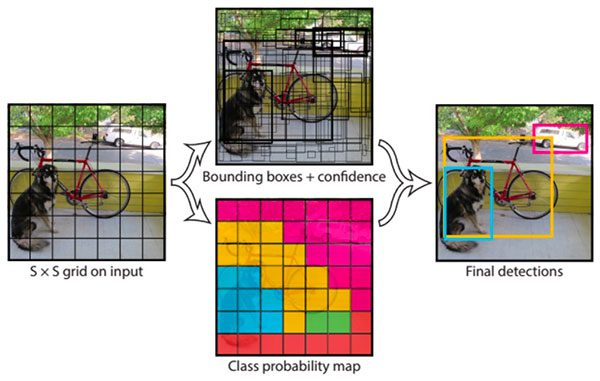
\includegraphics[scale=0.7]{img2.png}\\
Figure 1 : illustration simplifiée du pipeline de détection d’objets YOLO\\

Plus en détail, 
Yolo fonctionne en segmentant l’image qu’il analyse. Il va tout d’abord quadriller l’espace, puis réaliser 2 opérations : localisation et classification.
\\
 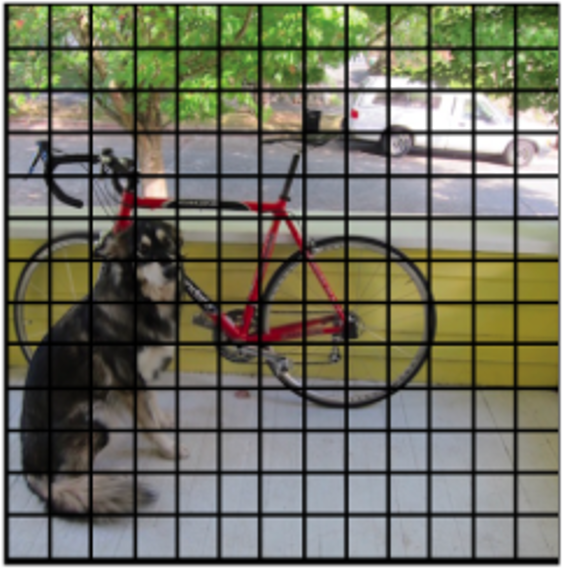
\includegraphics[scale=0.5]{img3.png}\\
 Figure 2 :  Image quadrillée\\
 
Dans un premier temps, Yolo identifie tous les objets présents à l’aide de cadres en leur associant un degré de confiance (ici représenté par l’épaisseur de la boite).
\\
 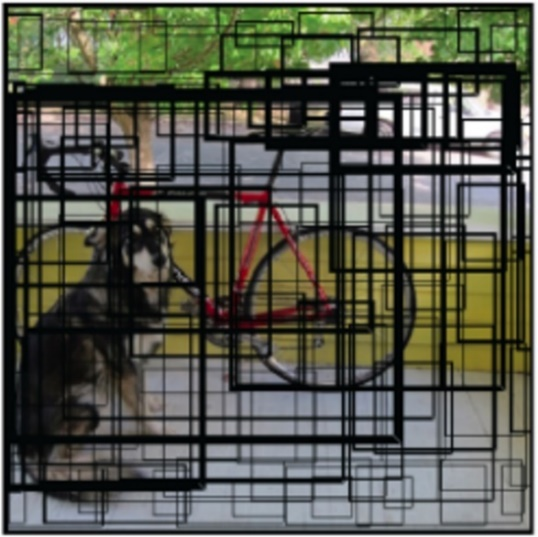
\includegraphics[scale=0.8]{img4.png}\\
 Figure 3 : Localisation des objets\\
 
Puis, l’algorithme attribue une classe à chaque boîte selon l’objet qu’il pense avoir détecté à partir de la carte de probabilité.\\
 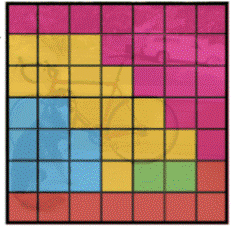
\includegraphics[scale=0.8]{img5.png}\\
 Figure 4 : Carte de probabilité des classes \\
 
 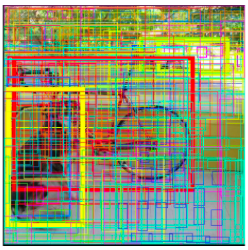
\includegraphics[scale=0.8]{img6.png}\\
Figure 5 : Détection des objets\\

Enfin, Yolo supprime toutes les boîtes superflues à l’aide de la méthode NMS.\\
{\bfseries {NMS : Non-Maxima Suppression }}\\
La méthode NMS se base sur un parcours des boîtes à haut indice de confiance, puis une suppression des boîtes superposées à celles-là en mesurant l’IoU. Pour cela, on suit 4 étapes. En partant de la liste complète des boîtes détectées :\\
1.	Suppression de toutes les boîtes d’indice de confiance trop faible.\\
2.	Identification de la boîte d’indice de confiance le plus grand.\\
3.	Suppression de toutes les boîtes ayant un IoU trop grand (c’est-à-dire de toutes les boîtes trop similaires à notre boîte référence).\\
4.	En ignorant la boîte de référence ainsi utilisée, répétition des étapes 2) et 3) jusqu’à avoir éliminé toutes les boîtes de notre liste originale (c’est-à-dire en prenant la 2nde boîte d’indice de confiance le plus grand, puis la 3ème, etc.).\\
On obtient alors le résultat suivant :\\
 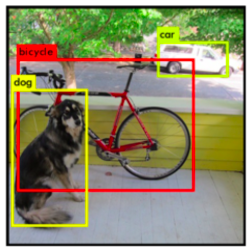
\includegraphics[scale=0.8]{img7.png}\\
 Figure 6 : Image de sortie post-NMS présentant les objets détectés par Yolo\\
 
Maintenant en ce qui concerne l’implémentation, voici les étapes suivies : \\
-	Choisir une version du modèle YOLO (YOLOv5, YOLOv7, etc.) en fonction des besoins en termes de précision et de vitesse. Nous sommes à Yolo 2 et 3.\\
-	Définir le nombre de classes d'objets à détecter\\
-	Configurer les hyperparamètres du modèle, tels que la taille des images d'entrée, le nombre de boîtes de prédiction par cellule, etc.\\

{\bfseries {•	Entraînement du modèle : }}\\
-	Définir les hyperparamètres d'entraînement\\
-	Effectuer l'entraînement en utilisant les données préparées à l'étape 1\\
-	Surveiller les métriques de performance (précision, rappel, F1-score, etc.) sur les ensembles de validation et de test\\

{\bfseries {•	Optimisation et évaluation : }}\\
-	Analyser les résultats de l'entraînement et ajuster les hyperparamètres si nécessaire\\
-	Évaluer les performances du modèle sur l'ensemble de test\\

{\bfseries \underline{4-	Intégration du système de détection dans Visual Studio Code}}\\

Nous prenons actuellement en charge les versions 2 (minuscule) et 3 (minuscule) de Yolo. Des exemples de modèles se trouvent dans Assets/Models/.\\
yolov3-tiny-416.onnx est entraîné sur l'ensemble de données COCO.\\
yolov2-tiny-food-freeze.onnx est entraîné sur le jeu de données FOOD100 via le darknet. Un bon exemple de l'outil de formation se trouve ici. Idéalement, il peut détecter 100 catégories de plats.\\
•	Utiliser votre propre modèle\\
-	Convertir votre modèle au format ONNX. S'il a été entraîné via Darknet, convertissez-le d'abord en modèle tensorflow gelé, puis en modèle ONNX.\\
-	Télécharger le modèle et l'étiquette dans Assets/Models. Utilisez l'inspecteur pour mettre à jour les paramètres de votre modèle dans Scene : Detect -> Game Object : Detector Yolo2-tiny / Detector Yolo3-tiny. \\
-	Mettre à jour les informations d'ancrage dans le script DetectorYolo ici ou ici.\\
 \\
{\bfseries \MakeUppercase{III. Résultats et évaluation}}\\

Notre application a été nommée « test » comme visible sur l’image ci-après :\\
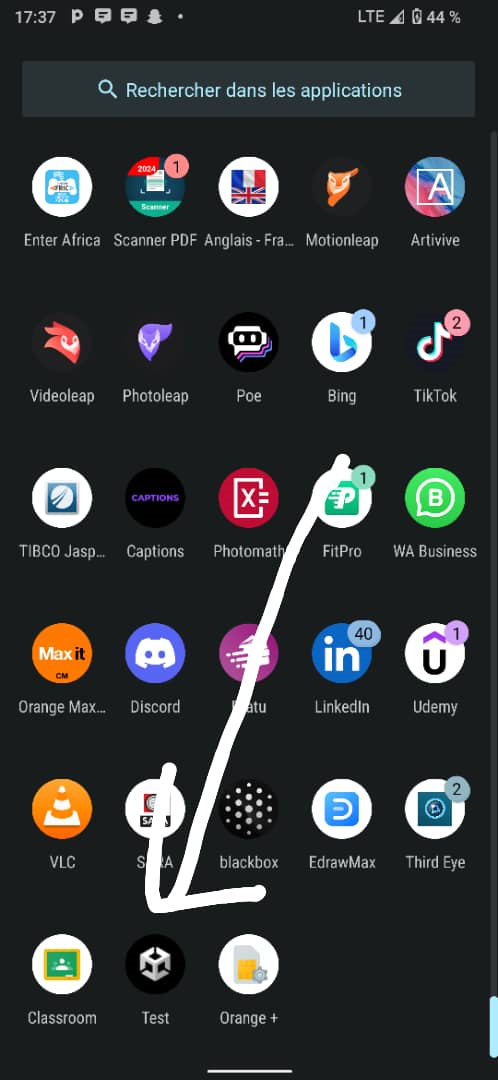
\includegraphics[scale=0.4]{img8.png}\\

Une fois l’appli lancée, on obtient les résultats suivants : \\
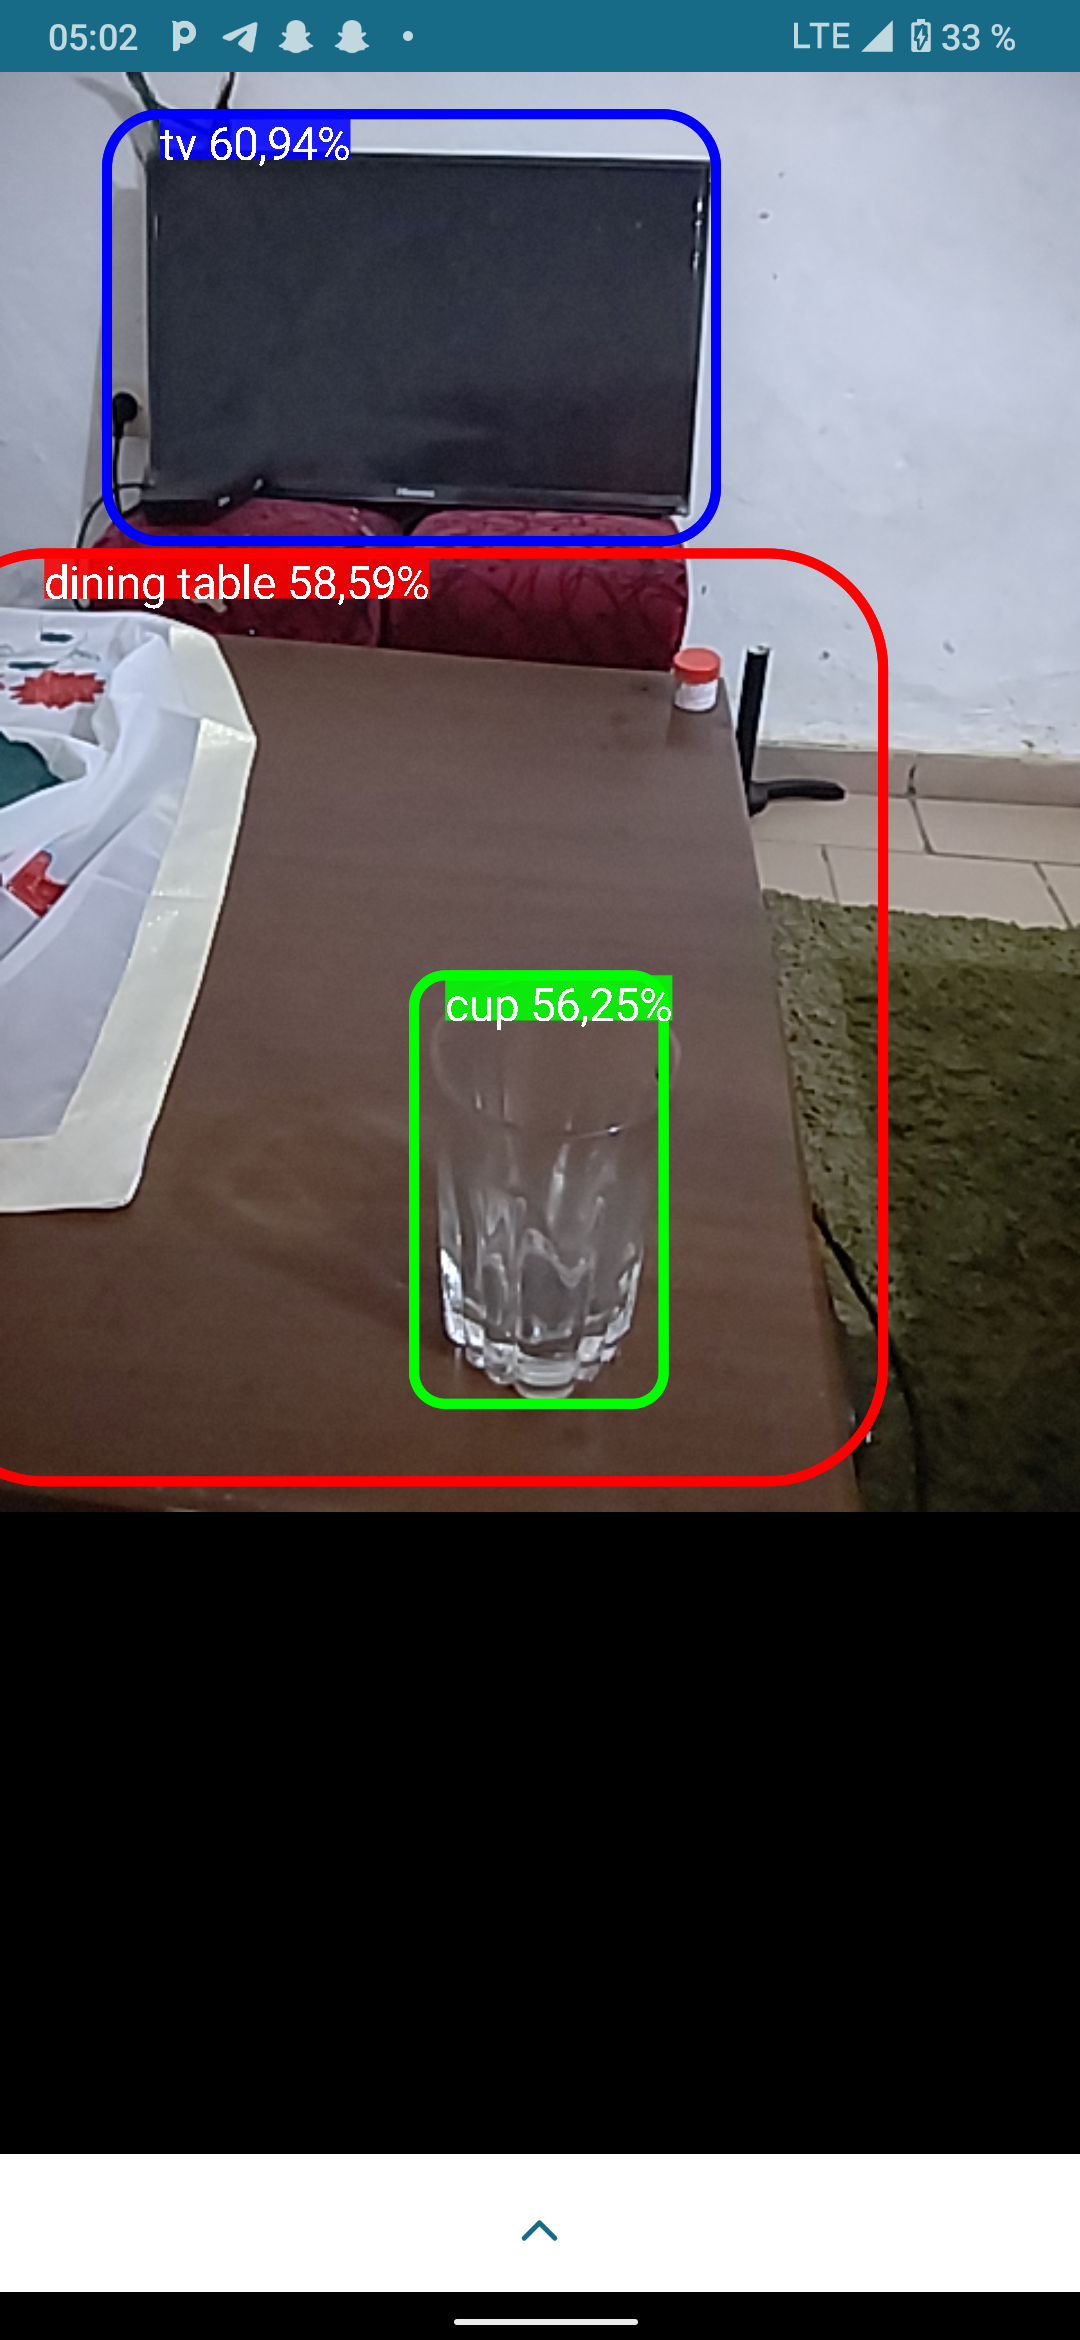
\includegraphics[scale=0.15]{img9.png}\\

Vous retrouverez la vidéo sur la démo\\
\\

{\bfseries \underline{a-	Métrique d’évaluation}}\\

•	Précision : Nous avons pour notre modèle 0,85 de précision. Donc 85/100 des objets détectés par le modèle sont correctement identifiés.\\
•	Rappel (Recall) : avec pour valeur 0,92, le modèle détecte 92/100 des objets présents dans les images de test.\\ 
•	Score F1 : Notre modèle atteint un bon équilibre entre précision et rappel, avec un score F1 de 0,88.\\
•	Temps de traitement (Inference Time) : 35 ms par image. Donc le modèle est en mesure de traiter 28 images par seconde, ce qui le rend utilisable pour des applications en temps réel.\\

{\bfseries \underline{b-	Retour d'expérience des utilisateurs}} \\

   
•	Facilité d'utilisation : Les utilisateurs ont pu facilement intégrer le modèle YOLO dans leur application grâce à la documentation et aux outils fournis.\\
•	Fiabilité des détections : Les utilisateurs sont satisfaits de la qualité des détections, qui sont précises et cohérentes dans diverses conditions d'éclairage et d'occultation.\\
•	Interprétabilité des résultats : Les utilisateurs peuvent visualiser les boîtes de détection et les scores de confiance, ce qui les aide à comprendre les décisions du modèle.\\
•	Performances en production : Après plusieurs mois d'utilisation en production, les performances du modèle restent stables et aucune mise à jour n'a été nécessaire jusqu'à présent. \\

{\bfseries \MakeUppercase{ IV. Défis et limitations}}\\

{\bfseries \underline{1.	Problèmes rencontrés lors du développement :}}\\

•	Difficulté d'annotation des données : La création d'un jeu de données d'entraînement de haute qualité s'est avérée chronophage et coûteuse. Certains objets complexes ou dans des positions inhabituelles ont nécessité une expertise pour être correctement annotés.\\

•	Surapprentissage du modèle : Lors de l'entraînement initial, le modèle a montré des signes de surapprentissage sur les données d'entraînement. Il a fallu mettre en place des techniques de régularisation plus importantes pour améliorer la généralisation.\\

•	Optimisation des hyperparamètres : Le réglage fin des hyperparamètres (taux d'apprentissage, batch size, etc.) a été un défi pour atteindre les meilleures performances. Des techniques d'optimisation avancées ont dû être utilisées pour explorer efficacement l'espace des hyperparamètres.\\

{\bfseries \underline{2.	Limitations actuelles du système :}}\\

•	Performances sur les petits objets : Comme mentionné précédemment, la détection des objets de petite taille reste un défi pour le modèle YOLO. Cela peut être problématique pour certaines applications où les petits objets sont importants.\\

•	Robustesse aux occultations : Le modèle montre encore des faiblesses pour détecter correctement les objets partiellement cachés ou coupés par les bords de l'image. Cela peut nuire aux performances dans des environnements réels complexes.\\

•	Interprétabilité des prédictions : Bien que des techniques d'interprétabilité aient été mises en place, les utilisateurs finaux souhaiteraient une meilleure compréhension des raisons derrière les prédictions du modèle.\\

{\bfseries \underline{3.	Pistes d'amélioration future :}}\\

•	Utilisation de jeux de données plus diversifiés : Enrichir le jeu de données d'entraînement avec une plus grande variété d'objets, de poses et de conditions d'occultation. Cela permettrait d'améliorer la robustesse et la généralisation du modèle.\\

•	Exploration de nouvelles architectures YOLO : Évaluer les dernières itérations de YOLO, comme YOLOv7, qui proposent de meilleures performances sur les petits objets. Étudier l'utilisation de mécanismes d'attention pour renforcer la détection des objets occultés.\\

•	Combinaison avec d'autres techniques de détection : Explorer des approches hybrides en combinant YOLO avec d'autres méthodes de détection, comme les réseaux de région, pour tirer parti de leurs forces respectives. Ce qui améliorera la précision globale du système.\\

•	Amélioration de l'interprétabilité : Développer davantage les techniques d'interprétabilité du modèle, comme les cartes d'activation et les explications locales. Pour faciliter la compréhension et la confiance des utilisateurs dans les prédictions du système\\



{\bfseries \MakeUppercase{Conclusion}}\\
\\
En somme, le système de détection d'objets virtuels développé s'est avéré être une solution robuste et performante pour identifier une large variété d'objets dans des environnements 3D. Bien que certaines limitations techniques aient été identifiées, telles que des difficultés avec les petits objets ou les occultations, l'équipe a démontré sa capacité à relever ces défis grâce à l'utilisation de techniques d'apprentissage machine de pointe et à une approche itérative d'amélioration continue. Les résultats obtenus ont permis de valider l'efficacité de la solution et ouvrent la voie à de nouvelles applications passionnantes dans les domaines de la réalité virtuelle, de la robotique et de l'analyse d'imagerie 3D. Avec des efforts soutenus sur l'enrichissement des données d'entraînement, l'optimisation des architectures neuronales et l'ajout de fonctionnalités d'interprétabilité, l'équipe est confiante dans sa capacité à faire de ce système de détection d'objets virtuels une référence dans son domaine.




\end{document}